% Q2: Normal Incidence Reflection and Transmission at a Media Boundary
% Teaching diagram: shows incident, reflected, and transmitted waves
\documentclass[border=10pt]{standalone}
\usepackage{tikz}
\usepackage{amsmath}
\usetikzlibrary{patterns, arrows.meta, decorations.pathreplacing}

\renewcommand{\familydefault}{\sfdefault}

\begin{document}
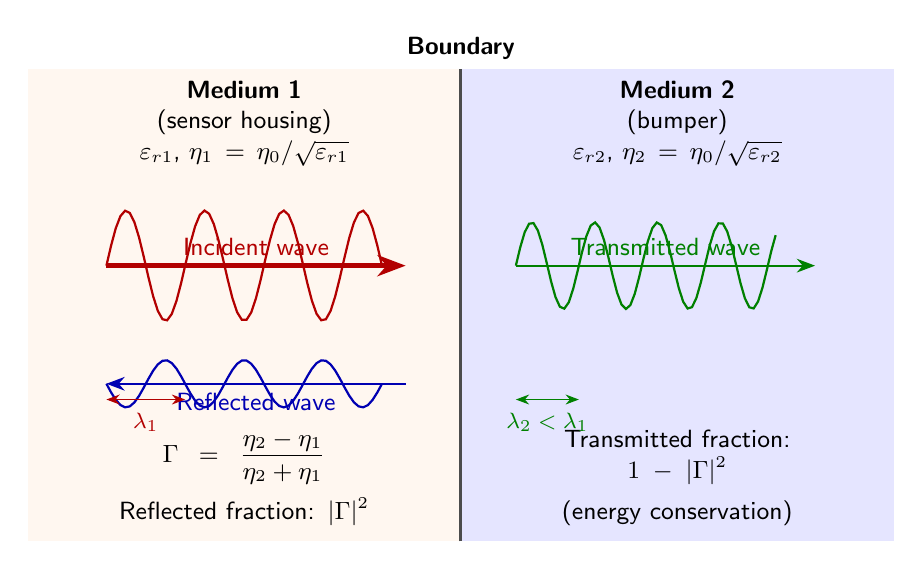
\begin{tikzpicture}[
    every node/.style={font=\sffamily\normalsize},
    >=Stealth
]

% --- Two media regions ---
\fill[orange!6] (0,0) rectangle (5.5,6);
\fill[blue!10] (5.5,0) rectangle (11,6);

% --- Boundary ---
\draw[very thick, black!70] (5.5,0) -- (5.5,6);
\node[above, font=\sffamily\small\bfseries] at (5.5,6) {Boundary};

% --- Medium labels ---
\node[font=\sffamily\small, text width=3.5cm, align=center] at (2.75,5.3)
    {\textbf{Medium 1}\\(sensor housing)\\$\varepsilon_{r1}$, $\eta_1 = \eta_0/\sqrt{\varepsilon_{r1}}$};
\node[font=\sffamily\small, text width=3.5cm, align=center] at (8.25,5.3)
    {\textbf{Medium 2}\\(bumper)\\$\varepsilon_{r2}$, $\eta_2 = \eta_0/\sqrt{\varepsilon_{r2}}$};

% --- Incident wave ---
\draw[->, ultra thick, red!70!black] (1,3.5) -- (4.8,3.5);
\node[above, font=\sffamily\small, red!70!black] at (2.9,3.5) {Incident wave};
\draw[thick, red!70!black, domain=1:4.5, samples=60]
    plot (\x, {3.5 + 0.7*sin(360*(\x-1)/1.0)});

% --- Reflected wave ---
\draw[->, thick, blue!70!black] (4.8,2.0) -- (1,2.0);
\node[below, font=\sffamily\small, blue!70!black] at (2.9,2.0) {Reflected wave};
\draw[thick, blue!70!black, domain=1:4.5, samples=60]
    plot (\x, {2.0 + 0.3*sin(360*(\x-1)/1.0 + 180)});

% --- Transmitted wave ---
\draw[->, thick, green!50!black] (6.2,3.5) -- (10,3.5);
\node[above, font=\sffamily\small, green!50!black] at (8.1,3.5) {Transmitted wave};
\draw[thick, green!50!black, domain=6.2:9.5, samples=60]
    plot (\x, {3.5 + 0.55*sin(360*(\x-6.2)/0.8)});

% --- Gamma annotation ---
\node[font=\sffamily\small, text width=4.5cm, align=center] at (2.75,0.8)
    {$\Gamma = \dfrac{\eta_2 - \eta_1}{\eta_2 + \eta_1}$\\[4pt]
     Reflected fraction: $|\Gamma|^2$};

\node[font=\sffamily\small, text width=4.5cm, align=center] at (8.25,0.8)
    {Transmitted fraction:\\$1 - |\Gamma|^2$\\[4pt]
     (energy conservation)};

% --- Wavelength comparison ---
\draw[<->, thin, red!70!black] (1, 1.8) -- (2, 1.8);
\node[below, font=\sffamily\footnotesize, red!70!black] at (1.5, 1.75) {$\lambda_1$};
\draw[<->, thin, green!50!black] (6.2, 1.8) -- (7.0, 1.8);
\node[below, font=\sffamily\footnotesize, green!50!black] at (6.6, 1.75) {$\lambda_2 < \lambda_1$};


\end{tikzpicture}
\end{document}
